\documentclass[11pt,a4paper]{article}

% ---------------------------------------------------------------------------
% M12x unit catalogue --- personal / research reference (not manuscript prose)
% Canonical design sources: mechanism_cards/, milestone1_part2_expanded_*.md
% Implementation: causal/experiments/handcrafted_m12x.py
% ---------------------------------------------------------------------------

\usepackage[margin=2.2cm]{geometry}
\usepackage{amsmath,amssymb}
\usepackage{booktabs}
\usepackage{array}
\usepackage{tabularx}
\usepackage{enumitem}
\usepackage{microtype}
\usepackage{xcolor}
\usepackage{tcolorbox}
\usepackage{tikz}
\usetikzlibrary{arrows.meta,positioning}
\usepackage{hyperref}
\hypersetup{colorlinks=true,linkcolor=black,urlcolor=blue!50!black,citecolor=black}

\newcolumntype{L}{>{\raggedright\arraybackslash}X}

% Compact DAG node style (do not use every node --- labels must stay text-only)
\tikzset{
  dag/.style={>=Stealth, every edge/.style={draw=black!80, thick, ->}},
  v/.style={
    circle, draw=black!75, thick, minimum size=7.2mm,
    inner sep=0pt, font=\sffamily\small
  },
  viso/.style={v, dashed, draw=black!45},
}

% Target callout
\newtcolorbox{targetbox}[1][]{%
  colback=blue!3!white,
  colframe=blue!40!black,
  coltitle=white,
  colbacktitle=blue!40!black,
  boxrule=0.6pt,
  left=4pt,right=4pt,top=3pt,bottom=3pt,
  fonttitle=\bfseries\sffamily\small,
  title=#1,
  before skip=0.6em,
  after skip=0.5em,
}

\newcommand{\unitmeta}[4]{%
  % #1 fixture key, #2 |S|, #3 rows, #4 targets
  \noindent
  \begin{tabularx}{\linewidth}{@{}l@{\hspace{1.2em}}L@{}}
    \textbf{Fixture key} & \texttt{#1}\\
    \textbf{Sources / rows} & $|S|=#2$ \quad$\Rightarrow$\quad $|\mathcal{D}|=#3$\\
    \textbf{Learning targets} & #4\\
  \end{tabularx}\par
  \vspace{0.35em}
}

\title{M12x Unit Catalogue\\[0.35em]
\large Graphs, mechanisms, tables, and reference hypotheses\\[0.25em]
\normalsize Expanded Milestone~1 Part~2 (U1--U7)}
\author{Causal ABA Learning project --- Samuel Waugh}
\date{Compiled from mechanism cards (redesign in progress, 2026-07-20)}

\begin{document}
\maketitle

\begin{abstract}
\noindent
Quick-reference catalogue of the seven accepted M12x units.
Each unit is a graph~$G$ together with a deterministic mechanism assignment
on every non-source.
Cells are
$(\text{unit},\,t\in N,\,\text{config}\in\{\text{ECAI},\text{AAMAS}\})$;
this document records inputs only (not learner outputs).
Units with several targets list each target separately, with its own
background-knowledge predictors, labels~$E^\pm$, and reference hypothesis
$\mathcal{H}_t^\star$.
\end{abstract}

\tableofcontents
\vspace{0.75em}
\noindent\rule{\linewidth}{0.4pt}

% ===========================================================================
\section{Shared regime}
\label{sec:regime}
% ===========================================================================

\begin{description}[style=nextline,leftmargin=1.6em,itemsep=0.25em]
  \item[Alphabet]
    $K=\{0,1,2\}$ for every variable.
  \item[DGP]
    Full source factorial over $K^{|S|}$, then propagate mechanisms in
    topological order.
    Mechanisms for multi-parent nodes are drawn from $\{\min,\max\}$.
    Single-parent maps may be unit-specific deterministic functions of the parent
    (U1: $\operatorname{copy}$; U4: asymmetric indicators).
    U5 uses the pilot curated $(x_0,x_1)$ support with $x_2:=\operatorname{copy}(x_1)$
    (not full source factorial; $x_1$ is not single-valued in $x_0$).
    U7 uses a curated diamond support (noisy fork arms; see~\S\ref{sec:u7}).
  \item[Labels (per target~$t$)]
    $E^+=\{t\neq 0\}$,\quad $E^-=\{t=0\}$
    (1-based sample ids on $\mathcal{D}$).
    Units may later override this per card; U1--U7 keep nonzero-positive.
  \item[Background knowledge]
    Every column except~$t$: exact-value predicates
    \texttt{*\_val\_0/1/2} only.
    No definitional \texttt{*\_nz} predicates.
    Descendants of~$t$ remain in BK as distractors; citing them in a learned
    rule is an explicit failure mode.
  \item[Reference hypothesis]
    Compact intensional rules in the \texttt{val} language
    (equationally: the parent conditions that separate $E^\pm$ on $\mathcal{D}$).
    U5/$t{=}x_1$ has no parent-aligned perfect $\mathcal{H}^\star$ (descendant only).
  \item[Cell count]
    7~units, 10~(unit, target) pairs, 20~cells after $\times\{\text{ECAI},\text{AAMAS}\}$.
\end{description}

\subsection*{At-a-glance}

\begin{center}
\small
\begin{tabular}{@{}clllcrr@{}}
\toprule
ID & Graph & Mechanisms & Targets~$N$ & $|S|$ & Rows & Cells \\
\midrule
U1 & separator (+ isolated $x_0$) & $x_2:=\operatorname{copy}(x_1)$ & $\{x_2\}$ & 2 & 9 & 2 \\
U2 & collider & $x_2:=\min(x_0,x_1)$ & $\{x_2\}$ & 2 & 9 & 2 \\
U3 & collider & $x_2:=\max(x_0,x_1)$ & $\{x_2\}$ & 2 & 9 & 2 \\
U4 & fork & $x_1:=2\cdot\mathbf{1}_{x_0\neq 2}$,\;$x_2:=2\cdot\mathbf{1}_{x_0\neq 0}$ & $\{x_1,x_2\}$ & 1 & 3 & 4 \\
U5 & chain & pilot $(x_0,x_1)$ support;\;$x_2:=\operatorname{copy}(x_1)$ & $\{x_1,x_2\}$ & 1 & 6 & 4 \\
U6 & Fabrizio G1 & $x_2:=\min$;\;$x_3:=x_1-x_2$ & $\{x_2,x_3\}$ & 2 & 9 & 4 \\
U7 & diamond & noisy fork arms;\;$x_3:=|x_1-x_2|$ & $\{x_3\}$ & 1 & 6 & 2 \\
\midrule
 & & & \textbf{10 targets} & & & \textbf{20} \\
\bottomrule
\end{tabular}
\end{center}

% ===========================================================================
\section{U1 --- Separator + copy}
\label{sec:u1}
% ===========================================================================

\unitmeta{m12\_u1\_separator\_copy}{2}{9}{$\{x_2\}$ (single target)}

\paragraph{Lesson.} Unique parent / copy with an isolated distractor.

\subsection{Graph}
\begin{center}
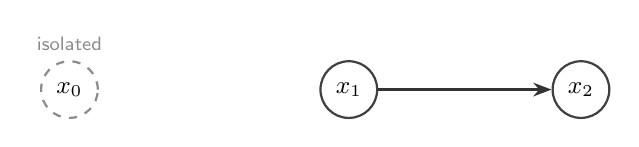
\begin{tikzpicture}[dag, node distance=18mm and 22mm]
  \node[viso, label={[font=\scriptsize\sffamily, text=black!45]above:isolated}] (x0) {$x_0$};
  \node[v, right=28mm of x0] (x1) {$x_1$};
  \node[v, right=of x1] (x2) {$x_2$};
  \path (x1) edge (x2);
\end{tikzpicture}
\end{center}
\noindent
$V=\{x_0,x_1,x_2\}$,\quad
$E=\{x_1\to x_2\}$,\quad
$S=\{x_0,x_1\}$,\quad
$N=\{x_2\}$.

\subsection{Mechanisms}
\[
  x_2 \;:=\; \operatorname{copy}(x_1).
\]
Isolated $x_0$ does not enter the mechanism.

\subsection{Table \texorpdfstring{$\mathcal{D}$}{D}}
Full factorial over $(x_0,x_1)$; then $x_2=x_1$.

\begin{center}
\small
\begin{tabular}{@{}rrrr@{}}
\toprule
id & $x_0$ & $x_1$ & $x_2=\operatorname{copy}(x_1)$ \\
\midrule
1 & 0 & 0 & 0 \\
2 & 0 & 1 & 1 \\
3 & 0 & 2 & 2 \\
4 & 1 & 0 & 0 \\
5 & 1 & 1 & 1 \\
6 & 1 & 2 & 2 \\
7 & 2 & 0 & 0 \\
8 & 2 & 1 & 1 \\
9 & 2 & 2 & 2 \\
\bottomrule
\end{tabular}
\end{center}

\subsection{Target \texorpdfstring{$t=x_2$}{t = x2}}
\begin{targetbox}[Single target --- sink]
Ancestors $\{x_1\}$; distractor $\{x_0\}$ (isolated, in BK); descendants $\emptyset$.\\
BK predictors: $x_0$, $x_1$ (exclude only $x_2$; \texttt{val} only, no \texttt{*\_nz}).\\
$E^+=\{2,3,5,6,8,9\}$ (6 rows, $x_2\neq 0$);\quad $E^-=\{1,4,7\}$ (3 rows, $x_2=0$).
\end{targetbox}

\noindent\textbf{Reference $\mathcal{H}_{x_2}^\star$:}
\begin{quote}\ttfamily\small
x2(A) :- x1\_val\_1(A).\\
x2(A) :- x1\_val\_2(A).
\end{quote}
\noindent\textit{Do not cite isolated $x_0$.}

% ===========================================================================
\section{U2 --- Collider + min}
\label{sec:u2}
% ===========================================================================

\unitmeta{m12\_u2\_collider\_min}{2}{9}{$\{x_2\}$ (single target)}

\paragraph{Lesson.} Conjunctive / both parents nonzero (min).

\subsection{Graph}
\begin{center}
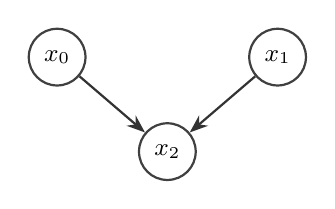
\begin{tikzpicture}[dag]
  \node[v] (x0) at (0,1.2) {$x_0$};
  \node[v] (x1) at (2.8,1.2) {$x_1$};
  \node[v] (x2) at (1.4,0) {$x_2$};
  \path (x0) edge (x2);
  \path (x1) edge (x2);
\end{tikzpicture}
\end{center}
\noindent
$V=\{x_0,x_1,x_2\}$,\quad
$E=\{x_0\to x_2,\; x_1\to x_2\}$,\quad
$S=\{x_0,x_1\}$,\quad
$N=\{x_2\}$.

\subsection{Mechanisms}
\[
  x_2 \;:=\; \min(x_0,x_1).
\]
On $\mathcal{D}$: $x_2\neq 0$ iff both parents are nonzero.

\subsection{Table \texorpdfstring{$\mathcal{D}$}{D}}
\begin{center}
\small
\begin{tabular}{@{}rrrr@{}}
\toprule
id & $x_0$ & $x_1$ & $x_2=\min$ \\
\midrule
1 & 0 & 0 & 0 \\
2 & 0 & 1 & 0 \\
3 & 0 & 2 & 0 \\
4 & 1 & 0 & 0 \\
5 & 1 & 1 & 1 \\
6 & 1 & 2 & 1 \\
7 & 2 & 0 & 0 \\
8 & 2 & 1 & 1 \\
9 & 2 & 2 & 2 \\
\bottomrule
\end{tabular}
\end{center}

\subsection{Target \texorpdfstring{$t=x_2$}{t = x2}}
\begin{targetbox}[Single target --- sink]
Ancestors $\{x_0,x_1\}$; other distractors $\emptyset$; descendants $\emptyset$.\\
BK predictors: $x_0$, $x_1$ (\texttt{val} only, no \texttt{*\_nz}).\\
$E^+=\{5,6,8,9\}$ (4 rows);\quad $E^-=\{1,2,3,4,7\}$ (5 rows).\\
On $\mathcal{D}$: $x_2\neq 0$ iff $x_0\neq 0$ and $x_1\neq 0$.
\end{targetbox}

\noindent\textbf{Reference $\mathcal{H}_{x_2}^\star$:}
\begin{quote}\ttfamily\small
x2(A) :- x0\_val\_1(A), x1\_val\_1(A).\\
x2(A) :- x0\_val\_1(A), x1\_val\_2(A).\\
x2(A) :- x0\_val\_2(A), x1\_val\_1(A).\\
x2(A) :- x0\_val\_2(A), x1\_val\_2(A).
\end{quote}

% ===========================================================================
\section{U3 --- Collider + max}
\label{sec:u3}
% ===========================================================================

\unitmeta{m12\_u3\_collider\_max}{2}{9}{$\{x_2\}$ (single target)}

\paragraph{Lesson.} Disjunctive / either parent nonzero (max).\\
\textit{Same edge set as U2; mechanism differs (max vs min).}

\subsection{Graph}
\begin{center}
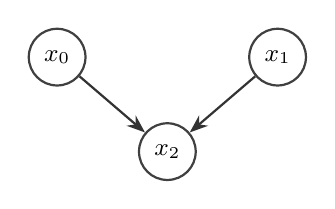
\begin{tikzpicture}[dag]
  \node[v] (x0) at (0,1.2) {$x_0$};
  \node[v] (x1) at (2.8,1.2) {$x_1$};
  \node[v] (x2) at (1.4,0) {$x_2$};
  \path (x0) edge (x2);
  \path (x1) edge (x2);
\end{tikzpicture}
\end{center}
\noindent
$V=\{x_0,x_1,x_2\}$,\quad
$E=\{x_0\to x_2,\; x_1\to x_2\}$,\quad
$S=\{x_0,x_1\}$,\quad
$N=\{x_2\}$.

\subsection{Mechanisms}
\[
  x_2 \;:=\; \max(x_0,x_1).
\]
On $\mathcal{D}$: $x_2\neq 0$ iff at least one parent is nonzero.

\subsection{Table \texorpdfstring{$\mathcal{D}$}{D}}
\begin{center}
\small
\begin{tabular}{@{}rrrr@{}}
\toprule
id & $x_0$ & $x_1$ & $x_2=\max$ \\
\midrule
1 & 0 & 0 & 0 \\
2 & 0 & 1 & 1 \\
3 & 0 & 2 & 2 \\
4 & 1 & 0 & 1 \\
5 & 1 & 1 & 1 \\
6 & 1 & 2 & 2 \\
7 & 2 & 0 & 2 \\
8 & 2 & 1 & 2 \\
9 & 2 & 2 & 2 \\
\bottomrule
\end{tabular}
\end{center}

\subsection{Target \texorpdfstring{$t=x_2$}{t = x2}}
\begin{targetbox}[Single target --- sink]
Ancestors $\{x_0,x_1\}$; other distractors $\emptyset$; descendants $\emptyset$.\\
BK predictors: $x_0$, $x_1$ (\texttt{val} only, no \texttt{*\_nz}).\\
$E^+=\{2,\ldots,9\}$ (8 rows);\quad $E^-=\{1\}$ (1 row).\\
On $\mathcal{D}$: $x_2\neq 0$ iff $x_0\neq 0$ or $x_1\neq 0$.
\end{targetbox}

\noindent\textbf{Reference $\mathcal{H}_{x_2}^\star$:}
\begin{quote}\ttfamily\small
x2(A) :- x0\_val\_1(A).\\
x2(A) :- x0\_val\_2(A).\\
x2(A) :- x1\_val\_1(A).\\
x2(A) :- x1\_val\_2(A).
\end{quote}

% ===========================================================================
\section{U4 --- Fork + asymmetric maps}
\label{sec:u4}
% ===========================================================================

\unitmeta{m12\_u4\_fork\_double\_copy}{1}{3}{%
  $\boldsymbol{\{x_1,\,x_2\}}$ --- \textbf{two targets} (asymmetric children)}

\paragraph{Lesson.} Parent vs sibling distractor (sibling correlated but imperfect).

\subsection{Graph}
\begin{center}
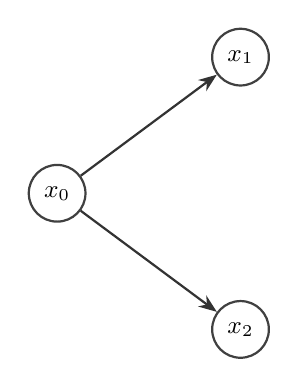
\begin{tikzpicture}[dag, node distance=14mm and 18mm]
  \node[v] (x0) {$x_0$};
  \node[v, above right=12mm and 18mm of x0] (x1) {$x_1$};
  \node[v, below right=12mm and 18mm of x0] (x2) {$x_2$};
  \path (x0) edge (x1);
  \path (x0) edge (x2);
\end{tikzpicture}
\end{center}
\noindent
$V=\{x_0,x_1,x_2\}$,\quad
$E=\{x_0\to x_1,\; x_0\to x_2\}$,\quad
$S=\{x_0\}$,\quad
$N=\{x_1,x_2\}$.

\subsection{Mechanisms}
\begin{align*}
  x_1 &\;:=\;
  \begin{cases}
    2 & \text{if } x_0\neq 2\\
    0 & \text{otherwise}
  \end{cases},\\
  x_2 &\;:=\;
  \begin{cases}
    2 & \text{if } x_0\neq 0\\
    0 & \text{otherwise}
  \end{cases}.
\end{align*}
Parent uniquely separates each child's nonzero labelling; sibling is imperfect.

\subsection{Table \texorpdfstring{$\mathcal{D}$}{D}}
\begin{center}
\small
\begin{tabular}{@{}rrrr@{}}
\toprule
id & $x_0$ & $x_1$ & $x_2$ \\
\midrule
1 & 0 & 2 & 0 \\
2 & 1 & 2 & 2 \\
3 & 2 & 0 & 2 \\
\bottomrule
\end{tabular}
\end{center}

% ----- target x1 -----
\subsection{Target \texorpdfstring{$t=x_1$}{t = x1}}
\begin{targetbox}[Target 1 of 2 --- child of $x_0$]
Ancestors $\{x_0\}$; sibling distractor $\{x_2\}$ (\textbf{in BK}); descendants $\emptyset$.\\
BK predictors: $x_0$, $x_2$ (\texttt{val} only, no \texttt{*\_nz}).\\
$E^+=\{1,2\}$;\quad $E^-=\{3\}$.\\
On $\mathcal{D}$: $x_1\neq 0$ iff $x_0\in\{0,1\}$.
\end{targetbox}

\noindent\textbf{Reference $\mathcal{H}_{x_1}^\star$:}
\begin{quote}\ttfamily\small
x1(A) :- x0\_val\_0(A).\\
x1(A) :- x0\_val\_1(A).
\end{quote}
\noindent\textit{Do not cite sibling $x_2$.}

% ----- target x2 -----
\subsection{Target \texorpdfstring{$t=x_2$}{t = x2}}
\begin{targetbox}[Target 2 of 2 --- child of $x_0$]
Ancestors $\{x_0\}$; sibling distractor $\{x_1\}$ (\textbf{in BK}); descendants $\emptyset$.\\
BK predictors: $x_0$, $x_1$ (\texttt{val} only, no \texttt{*\_nz}).\\
$E^+=\{2,3\}$;\quad $E^-=\{1\}$.\\
On $\mathcal{D}$: $x_2\neq 0$ iff $x_0\neq 0$.
\end{targetbox}

\noindent\textbf{Reference $\mathcal{H}_{x_2}^\star$:}
\begin{quote}\ttfamily\small
x2(A) :- x0\_val\_1(A).\\
x2(A) :- x0\_val\_2(A).
\end{quote}
\noindent\textit{Do not cite sibling $x_1$.}

% ===========================================================================
\section{U5 --- Chain + correlated ancestor (pilot)}
\label{sec:u5}
% ===========================================================================

\unitmeta{m12\_u5\_chain\_double\_copy}{1}{6}{%
  $\boldsymbol{\{x_1,\,x_2\}}$ --- \textbf{two targets} (intermediate + sink)}

\paragraph{Lesson.} Parent vs correlated ancestor (sink); descendant-in-BK when learning the intermediate.

\subsection{Graph}
\begin{center}
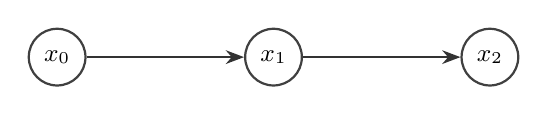
\begin{tikzpicture}[dag, node distance=20mm]
  \node[v] (x0) {$x_0$};
  \node[v, right=of x0] (x1) {$x_1$};
  \node[v, right=of x1] (x2) {$x_2$};
  \path (x0) edge (x1);
  \path (x1) edge (x2);
\end{tikzpicture}
\end{center}
\noindent
$V=\{x_0,x_1,x_2\}$,\quad
$E=\{x_0\to x_1,\; x_1\to x_2\}$,\quad
$S=\{x_0\}$,\quad
$N=\{x_1,x_2\}$.

\subsection{Mechanisms}
For each $x_0\in K$, include pairs
$(x_0,x_1)=(x_0,x_0)$ and $(x_0,(x_0+1)\bmod 3)$; then
\begin{equation*}
  x_2 \;:=\; \operatorname{copy}(x_1).
\end{equation*}
Not full source factorial: $x_1$ is not a single-valued function of $x_0$.
Parent $x_1$ uniquely separates nonzero labelling of $x_2$; ancestor $x_0$ is imperfect.

\subsection{Table \texorpdfstring{$\mathcal{D}$}{D}}
\begin{center}
\small
\begin{tabular}{@{}rrrr@{}}
\toprule
id & $x_0$ & $x_1$ & $x_2=\operatorname{copy}(x_1)$ \\
\midrule
1 & 0 & 0 & 0 \\
2 & 0 & 1 & 1 \\
3 & 1 & 1 & 1 \\
4 & 1 & 2 & 2 \\
5 & 2 & 2 & 2 \\
6 & 2 & 0 & 0 \\
\bottomrule
\end{tabular}
\end{center}

% ----- target x1 -----
\subsection{Target \texorpdfstring{$t=x_1$}{t = x1} (intermediate)}
\begin{targetbox}[Target 1 of 2 --- intermediate; descendant distractor cell]
Ancestors $\{x_0\}$ (imperfect under nonzero labelling); other distractors $\emptyset$;
descendants $\{x_2\}$ (\textbf{in BK}; citing = failure mode).\\
BK predictors: $x_0$, $x_2$ (\texttt{val} only, no \texttt{*\_nz}).\\
$E^+=\{2,3,4,5\}$;\quad $E^-=\{1,6\}$.\\
On $\mathcal{D}$: $x_1\neq 0$ iff $x_2\neq 0$ (because $x_2=x_1$).
\end{targetbox}

\noindent\textbf{Reference $\mathcal{H}_{x_1}^\star$:}
\textit{None (parent-aligned).}
No perfect \texttt{x0\_val\_*} separator.
Descendant rules are extensionally perfect but are \textbf{not} $\mathcal{H}^\star$.

% ----- target x2 -----
\subsection{Target \texorpdfstring{$t=x_2$}{t = x2} (sink)}
\begin{targetbox}[Target 2 of 2 --- sink; parent vs ancestor]
Ancestors $\{x_0,x_1\}$ (parent $x_1$ preferred; $x_0$ correlated but imperfect);
descendants $\emptyset$.\\
BK predictors: $x_0$, $x_1$ (\texttt{val} only, no \texttt{*\_nz}).\\
$E^+=\{2,3,4,5\}$;\quad $E^-=\{1,6\}$.\\
On $\mathcal{D}$: $x_2\neq 0$ iff $x_1\in\{1,2\}$.
\end{targetbox}

\noindent\textbf{Reference $\mathcal{H}_{x_2}^\star$ (direct parent):}
\begin{quote}\ttfamily\small
x2(A) :- x1\_val\_1(A).\\
x2(A) :- x1\_val\_2(A).
\end{quote}
\noindent
\textit{Note:} no \texttt{x0\_val\_*}-only rule set matches this labelling perfectly.
Ancestor citation is a parent-vs-ancestor divergence, not the reference.

% ===========================================================================
\section{U6 --- Fabrizio G1 + min then difference}
\label{sec:u6}
% ===========================================================================

\unitmeta{m12\_u6\_g1\_and\_cone}{2}{9}{%
  $\boldsymbol{\{x_2,\,x_3\}}$ --- \textbf{two targets} (intermediate + sink)}

\paragraph{Lesson.} Four-node G1; intermediate min (both parents); sink
$x_3\neq 0\iff x_1>x_2$ needs both $\mathrm{Pa}(x_3)$; imperfect descendant distractor.\\
\textit{Graph provenance:} Fabrizio G1
(\texttt{ArgCausalDisco} four-node example).
Mechanisms/DGP are project-chosen.

\subsection{Graph}
\begin{center}
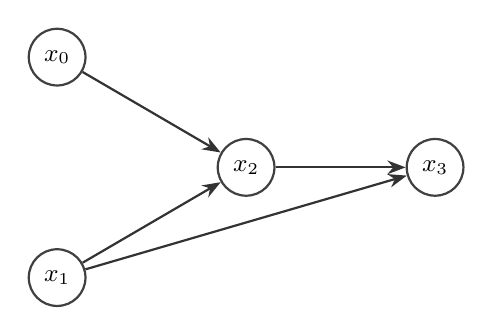
\begin{tikzpicture}[dag]
  \node[v] (x0) at (0,1.4) {$x_0$};
  \node[v] (x1) at (0,-1.4) {$x_1$};
  \node[v] (x2) at (2.4,0) {$x_2$};
  \node[v] (x3) at (4.8,0) {$x_3$};
  \path (x0) edge (x2);
  \path (x1) edge (x2);
  \path (x1) edge (x3);
  \path (x2) edge (x3);
\end{tikzpicture}
\end{center}
\noindent
$V=\{x_0,x_1,x_2,x_3\}$,\quad
$E=\{x_0\to x_2,\; x_1\to x_2,\; x_1\to x_3,\; x_2\to x_3\}$,\\
$S=\{x_0,x_1\}$,\quad
$N=\{x_2,x_3\}$,\quad
$\mathrm{Pa}(x_2)=\{x_0,x_1\}$,\quad
$\mathrm{Pa}(x_3)=\{x_1,x_2\}$.

\subsection{Mechanisms}
\begin{align*}
  x_2 &\;:=\; \min(x_0,x_1),\\
  x_3 &\;:=\; x_1-x_2.
\end{align*}
On $\mathcal{D}$, $x_2\le x_1$, so $x_3\in\{0,1,2\}$.
Sink nonzero labelling: $x_3\neq 0$ iff $x_1>x_2$ (both parents required).
No $x_3\equiv x_2$ or $x_3\equiv x_1$ collapse.

\subsection{Table \texorpdfstring{$\mathcal{D}$}{D}}
\begin{center}
\small
\begin{tabular}{@{}rrrrr@{}}
\toprule
id & $x_0$ & $x_1$ & $x_2=\min(x_0,x_1)$ & $x_3=x_1-x_2$ \\
\midrule
1 & 0 & 0 & 0 & 0 \\
2 & 0 & 1 & 0 & 1 \\
3 & 0 & 2 & 0 & 2 \\
4 & 1 & 0 & 0 & 0 \\
5 & 1 & 1 & 1 & 0 \\
6 & 1 & 2 & 1 & 1 \\
7 & 2 & 0 & 0 & 0 \\
8 & 2 & 1 & 1 & 0 \\
9 & 2 & 2 & 2 & 0 \\
\bottomrule
\end{tabular}
\end{center}

% ----- target x2 -----
\subsection{Target \texorpdfstring{$t=x_2$}{t = x2} (intermediate)}
\begin{targetbox}[Target 1 of 2 --- intermediate; descendant $x_3$ in BK]
Ancestors $\{x_0,x_1\}$; descendants $\{x_3\}$ (\textbf{in BK}; citing = failure mode).\\
BK predictors: $x_0$, $x_1$, $x_3$ (\texttt{val} only, no \texttt{*\_nz}).\\
$E^+=\{5,6,8,9\}$ (4);\quad $E^-=\{1,2,3,4,7\}$ (5).\\
On $\mathcal{D}$: $x_2\neq 0$ iff $x_0\neq 0$ and $x_1\neq 0$.
Descendant $x_3\neq 0$ only on $\{2,3,6\}$ (imperfect separator).
\end{targetbox}

\noindent\textbf{Reference $\mathcal{H}_{x_2}^\star$:}
\begin{quote}\ttfamily\small
x2(A) :- x0\_val\_1(A), x1\_val\_1(A).\\
x2(A) :- x0\_val\_1(A), x1\_val\_2(A).\\
x2(A) :- x0\_val\_2(A), x1\_val\_1(A).\\
x2(A) :- x0\_val\_2(A), x1\_val\_2(A).
\end{quote}
\noindent\textit{Must not cite descendant $x_3$.}

% ----- target x3 -----
\subsection{Target \texorpdfstring{$t=x_3$}{t = x3} (sink)}
\begin{targetbox}[Target 2 of 2 --- sink; $x_1>x_2$]
Ancestors $\{x_0,x_1,x_2\}$; parents $\{x_1,x_2\}$; descendants $\emptyset$.\\
BK predictors: $x_0$, $x_1$, $x_2$ (\texttt{val} only, no \texttt{*\_nz}).\\
$E^+=\{2,3,6\}$ (3);\quad $E^-=\{1,4,5,7,8,9\}$ (6).\\
On $\mathcal{D}$: $x_3\neq 0$ iff $x_1>x_2$ (neither parent alone separates).
\end{targetbox}

\noindent\textbf{Reference $\mathcal{H}_{x_3}^\star$ (parent-based):}
\begin{quote}\ttfamily\small
x3(A) :- x1\_val\_1(A), x2\_val\_0(A).\\
x3(A) :- x1\_val\_2(A), x2\_val\_0(A).\\
x3(A) :- x1\_val\_2(A), x2\_val\_1(A).
\end{quote}

% ===========================================================================
\section{U7 --- Diamond + noisy fork arms}
\label{sec:u7}
% ===========================================================================

\unitmeta{m12\_u7\_g1\_or\_cone}{1}{6}{%
  $\{x_3\}$ (single target --- sink)}

\paragraph{Lesson.} Both-parent sink when parents are correlated siblings; root and each
sibling alone imperfect (U5-style curated noisy arms).

\subsection{Graph}
\begin{center}
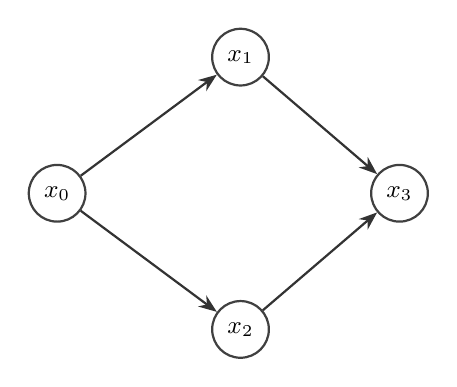
\begin{tikzpicture}[dag, node distance=14mm and 18mm]
  \node[v] (x0) {$x_0$};
  \node[v, above right=12mm and 18mm of x0] (x1) {$x_1$};
  \node[v, below right=12mm and 18mm of x0] (x2) {$x_2$};
  \node[v, right=36mm of x0] (x3) {$x_3$};
  \path (x0) edge (x1);
  \path (x0) edge (x2);
  \path (x1) edge (x3);
  \path (x2) edge (x3);
\end{tikzpicture}
\end{center}
\noindent
$V=\{x_0,x_1,x_2,x_3\}$,\quad
$E=\{x_0\to x_1,\; x_0\to x_2,\; x_1\to x_3,\; x_2\to x_3\}$,\\
$S=\{x_0\}$,\quad
$N=\{x_1,x_2,x_3\}$,\quad
$\mathrm{Pa}(x_3)=\{x_1,x_2\}$.

\subsection{Mechanisms}
For each $x_0\in K$: $x_1:=(x_0+1)\bmod 3$; two $x_2$ values
$(x_0+2)\bmod 3$ (differ) and $x_1$ (collapse); then
\begin{equation*}
  x_3 \;:=\; |x_1-x_2|.
\end{equation*}
Not full source factorial. On $\mathcal{D}$: $x_3\neq 0$ iff $x_1\neq x_2$.
No singleton among $\{x_0,x_1,x_2\}$ is a perfect \texttt{val}-union separator of $E^\pm$.

\subsection{Table \texorpdfstring{$\mathcal{D}$}{D}}
\begin{center}
\small
\begin{tabular}{@{}rrrrr@{}}
\toprule
id & $x_0$ & $x_1$ & $x_2$ & $x_3=|x_1-x_2|$ \\
\midrule
1 & 0 & 1 & 2 & 1 \\
2 & 0 & 1 & 1 & 0 \\
3 & 1 & 2 & 0 & 2 \\
4 & 1 & 2 & 2 & 0 \\
5 & 2 & 0 & 1 & 1 \\
6 & 2 & 0 & 0 & 0 \\
\bottomrule
\end{tabular}
\end{center}

\subsection{Target \texorpdfstring{$t=x_3$}{t = x3} (sink)}
\begin{targetbox}[Single target --- both sibling parents]
Ancestors $\{x_0,x_1,x_2\}$; parents $\{x_1,x_2\}$; descendants $\emptyset$.\\
BK predictors: $x_0$, $x_1$, $x_2$ (\texttt{val} only, no \texttt{*\_nz}).\\
$E^+=\{1,3,5\}$;\quad $E^-=\{2,4,6\}$.\\
On $\mathcal{D}$: $x_3\neq 0$ iff $x_1\neq x_2$.
\end{targetbox}

\noindent\textbf{Reference $\mathcal{H}_{x_3}^\star$:}
\begin{quote}\ttfamily\small
x3(A) :- x1\_val\_1(A), x2\_val\_2(A).\\
x3(A) :- x1\_val\_2(A), x2\_val\_0(A).\\
x3(A) :- x1\_val\_0(A), x2\_val\_1(A).
\end{quote}

% ===========================================================================
\section*{Source pointers}
% ===========================================================================

\begin{description}[leftmargin=1.4em,style=nextline,itemsep=0.2em]
  \item[Mechanism cards]
    \texttt{docs/research/milestone\_plans/milestone1\_part2/mechanism\_cards/}
  \item[Unit set]
    \texttt{milestone1\_part2\_expanded\_unit\_set.md}
  \item[Approach]
    \texttt{milestone1\_part2\_expanded\_approach.md}
  \item[Implementation]
    \texttt{causal/experiments/handcrafted\_m12x.py}
\end{description}

\end{document}
